
\documentclass[border=10pt, 12pt]{standalone}
\usepackage[svgnames]{xcolor}
\usepackage{amsmath}
\usepackage{pgfplots}
\pgfplotsset{compat=newest}
\usepackage[sfdefault]{FiraSans}
\usepackage{FiraMono}
\renewcommand*\familydefault{\sfdefault}
\begin{document}
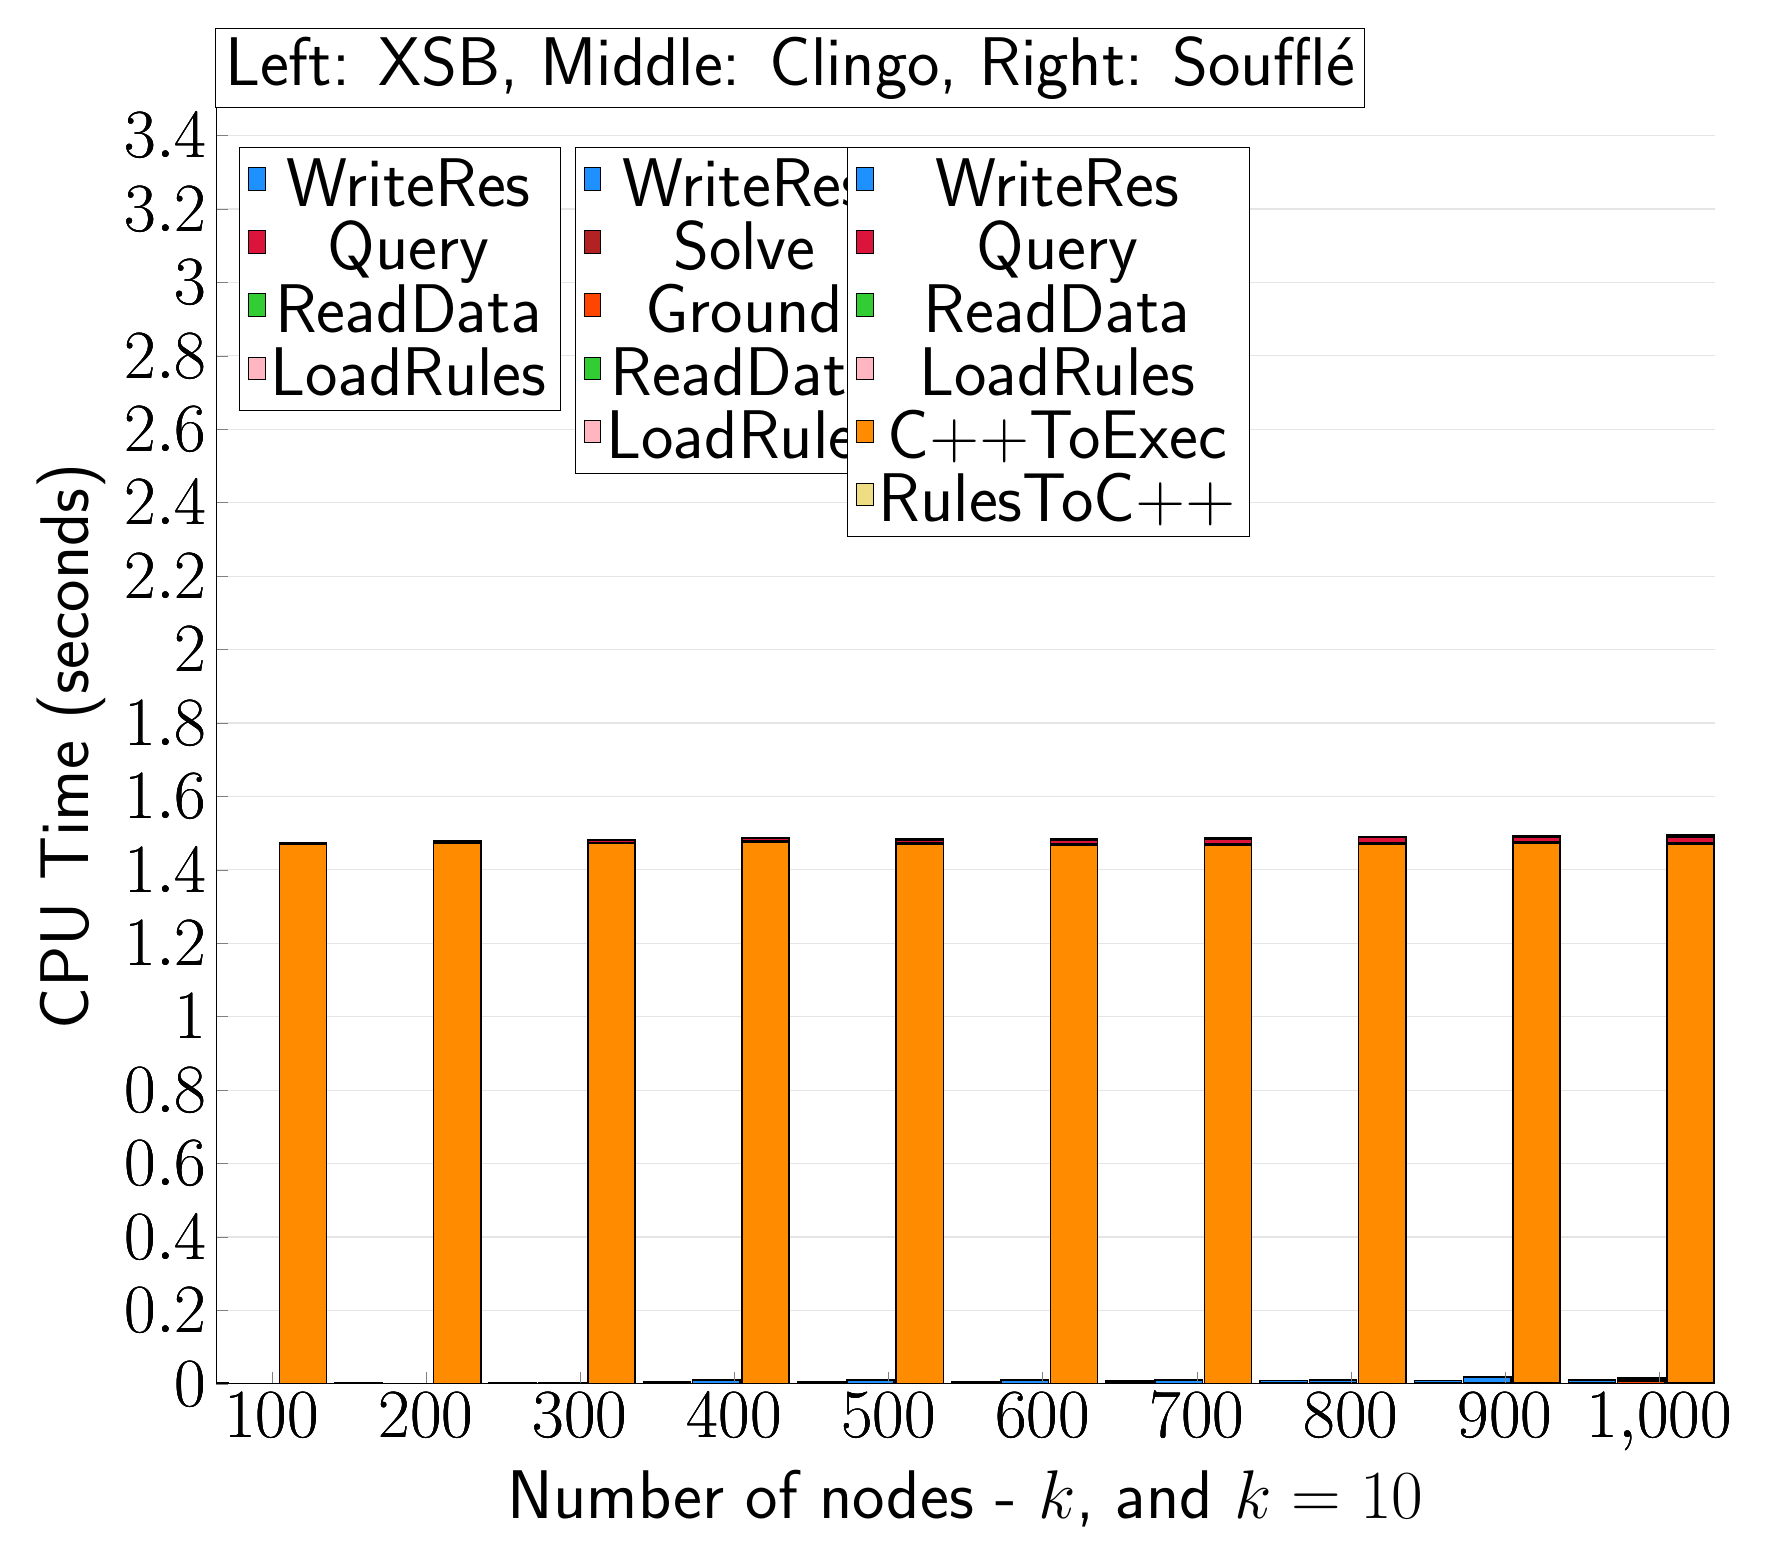
\begin{tikzpicture}
                        \begin{axis}[bar shift=-24.3pt, 
   ybar stacked,
   width=1.7\textwidth,
   bar width=0.6cm,
   ymajorgrids, tick align=inside,
   major grid style={draw=gray!20},
   xtick=data,
   ymin=0, ymax=3.4739999999999998,
   axis x line*=bottom,
   axis y line*=left,
   enlarge x limits=0.04,
   legend style={
       at={(0.23, 0.97)},
       anchor=north east,
       legend columns=1,
       font=\Huge,
   },
   ylabel={CPU Time (seconds)},
   xlabel={Number of nodes - $k$, and $k=10$},
   label style={font=\Huge},
   tick label style={font=\Huge},
]
\addlegendimage{fill=DodgerBlue, draw=black, line width=0.2pt}
\addlegendentry{WriteRes}
\addlegendimage{fill=Crimson, draw=black, line width=0.2pt}
\addlegendentry{Query}
\addlegendimage{fill=LimeGreen, draw=black, line width=0.2pt}
\addlegendentry{ReadData}
\addlegendimage{fill=LightPink, draw=black, line width=0.2pt}
\addlegendentry{LoadRules}
\addplot +[fill=LightPink, draw=black, line width=0.55pt] coordinates {
(100, 0.0005503999999999997)
(200, 0.0005562)
(300, 0.0005492000000000008)
(400, 0.0005512000000000004)
(500, 0.0005535999999999998)
(600, 0.0005523999999999998)
(700, 0.0005494000000000001)
(800, 0.0005576000000000005)
(900, 0.0005543999999999999)
(1000, 0.0005580000000000003)
};
\addplot +[fill=LimeGreen, draw=black, line width=0.55pt] coordinates {
(100, 0.00020540000000000038)
(200, 0.0002884000000000002)
(300, 0.0003651999999999996)
(400, 0.0004458)
(500, 0.0005207999999999999)
(600, 0.0006035999999999999)
(700, 0.0006795999999999996)
(800, 0.0007524)
(900, 0.0008414000000000002)
(1000, 0.0009302000000000002)
};
\addplot +[fill=Crimson, draw=black, line width=0.55pt] coordinates {
(100, 0.00010319999999999966)
(200, 0.00019299999999999997)
(300, 0.0003006)
(400, 0.0004002000000000002)
(500, 0.0005012)
(600, 0.0006108000000000001)
(700, 0.0006798000000000006)
(800, 0.0008136000000000006)
(900, 0.0008901999999999995)
(1000, 0.0009993999999999992)
};
\addplot +[fill=DodgerBlue, draw=black, line width=0.55pt] coordinates {
(100, 0.0009050000000000004)
(200, 0.0017158)
(300, 0.0025024000000000005)
(400, 0.0033445999999999997)
(500, 0.004117600000000001)
(600, 0.004911799999999999)
(700, 0.0057821999999999995)
(800, 0.0065138)
(900, 0.0073628)
(1000, 0.0081762)
};
\end{axis}

\begin{axis}[bar shift=-6.5pt, 
   ybar stacked,
   width=1.7\textwidth,
   bar width=0.6cm,
   ymajorgrids, tick align=inside,
   major grid style={draw=none},
   xtick=data,
   ymin=0, ymax=3.4739999999999998,
   axis x line*=none,
   axis y line*=none,
   enlarge x limits=0.04,
   legend style={
       at={(0.454, 0.97)},
       anchor=north east,
       legend columns=1,
       font=\Huge,
   },
   label style={font=\Huge},
   tick label style={font=\Huge},
]
\addlegendimage{fill=DodgerBlue, draw=black, line width=0.2pt}
\addlegendentry{WriteRes}
\addlegendimage{fill=FireBrick, draw=black, line width=0.2pt}
\addlegendentry{Solve}
\addlegendimage{fill=OrangeRed, draw=black, line width=0.2pt}
\addlegendentry{Ground}
\addlegendimage{fill=LimeGreen, draw=black, line width=0.2pt}
\addlegendentry{ReadData}
\addlegendimage{fill=LightPink, draw=black, line width=0.2pt}
\addlegendentry{LoadRules}
\addplot +[fill=LightPink, draw=black, line width=0.55pt] coordinates {
(100, 0.0)
(200, 0.0)
(300, 0.0)
(400, 0.0)
(500, 0.0)
(600, 0.0)
(700, 0.0)
(800, 0.0)
(900, 0.0)
(1000, 0.0)
};
\addplot +[fill=LimeGreen, draw=black, line width=0.55pt] coordinates {
(100, 0.0)
(200, 0.0)
(300, 0.0)
(400, 0.0)
(500, 0.0)
(600, 0.0)
(700, 0.0)
(800, 0.0)
(900, 0.0)
(1000, 0.0)
};
\addplot +[fill=OrangeRed, draw=black, line width=0.55pt] coordinates {
(100, 0.0)
(200, 0.0)
(300, 0.0)
(400, 0.0)
(500, 0.0)
(600, 0.0)
(700, 0.0)
(800, 0.0)
(900, 0.0020000000000000018)
(1000, 0.006000000000000005)
};
\addplot +[fill=FireBrick, draw=black, line width=0.55pt] coordinates {
(100, 0.0)
(200, 0.0)
(300, 0.0)
(400, 0.0)
(500, 0.0)
(600, 0.0)
(700, 0.0)
(800, 0.0020000000000000018)
(900, 0.0020000000000000018)
(1000, 0.0040000000000000036)
};
\addplot +[fill=DodgerBlue, draw=black, line width=0.55pt] coordinates {
(100, 0.0)
(200, 0.0)
(300, 0.0020000000000000018)
(400, 0.010000000000000009)
(500, 0.010000000000000009)
(600, 0.010000000000000009)
(700, 0.010000000000000009)
(800, 0.008000000000000007)
(900, 0.014000000000000012)
(1000, 0.006000000000000005)
};
\end{axis}

\begin{axis}[bar shift=11.3pt, 
   ybar stacked,
   width=1.7\textwidth,
   bar width=0.6cm,
   ymajorgrids, tick align=inside,
   major grid style={draw=none},
   xtick=data,
   ymin=0, ymax=3.4739999999999998,
   axis x line*=none,
   axis y line*=none,
   enlarge x limits=0.04,
   legend style={
       at={(0.69, 0.97)},
       anchor=north east,
       legend columns=1,
       font=\Huge,
   },
   label style={font=\Huge},
   tick label style={font=\Huge},
]
\addlegendimage{fill=DodgerBlue, draw=black, line width=0.2pt}
\addlegendentry{WriteRes}
\addlegendimage{fill=Crimson, draw=black, line width=0.2pt}
\addlegendentry{Query}
\addlegendimage{fill=LimeGreen, draw=black, line width=0.2pt}
\addlegendentry{ReadData}
\addlegendimage{fill=LightPink, draw=black, line width=0.2pt}
\addlegendentry{LoadRules}
\addlegendimage{fill=DarkOrange, draw=black, line width=0.2pt}
\addlegendentry{C++ToExec}
\addlegendimage{fill=LightGoldenrod, draw=black, line width=0.2pt}
\addlegendentry{RulesToC++}
\addplot +[fill=LightGoldenrod, draw=black, line width=0.55pt] coordinates {
(100, 0.0)
(200, 0.0)
(300, 0.0)
(400, 0.0)
(500, 0.0)
(600, 0.0)
(700, 0.0)
(800, 0.0)
(900, 0.004000000000000001)
(1000, 0.0020000000000000005)
};
\addplot +[fill=DarkOrange, draw=black, line width=0.55pt] coordinates {
(100, 1.4700000000000002)
(200, 1.472)
(300, 1.472)
(400, 1.4760000000000002)
(500, 1.47)
(600, 1.468)
(700, 1.4679999999999997)
(800, 1.47)
(900, 1.468)
(1000, 1.4679999999999997)
};
\addplot +[fill=LightPink, draw=black, line width=0.55pt] coordinates {
(100, 0.00016639999999999998)
(200, 0.0001746)
(300, 0.0001682)
(400, 0.0001662)
(500, 0.0001818)
(600, 0.0001728)
(700, 0.0001706)
(800, 0.00018360000000000002)
(900, 0.0001744)
(1000, 0.0001694)
};
\addplot +[fill=LimeGreen, draw=black, line width=0.55pt] coordinates {
(100, 0.0008546)
(200, 0.001211)
(300, 0.0016538)
(400, 0.0020718)
(500, 0.002424)
(600, 0.0027264000000000004)
(700, 0.0030444)
(800, 0.0035477999999999994)
(900, 0.0033313999999999996)
(1000, 0.0041838)
};
\addplot +[fill=Crimson, draw=black, line width=0.55pt] coordinates {
(100, 0.0022238)
(200, 0.0039704)
(300, 0.00598)
(400, 0.00779)
(500, 0.009280199999999999)
(600, 0.0097022)
(700, 0.011700799999999999)
(800, 0.0138316)
(900, 0.01305)
(1000, 0.015516600000000002)
};
\addplot +[fill=DodgerBlue, draw=black, line width=0.55pt] coordinates {
(100, 0.001306)
(200, 0.0016687999999999998)
(300, 0.0018242000000000002)
(400, 0.0017274)
(500, 0.0026190000000000002)
(600, 0.0033908000000000002)
(700, 0.003269)
(800, 0.0038314)
(900, 0.0038378)
(1000, 0.0044506)
};
\end{axis}


\node[anchor=south, draw, fill=white] at (rel axis cs:0.42, 1) {\Huge Left: XSB, Middle: Clingo, Right: Soufflé};
\end{tikzpicture}
\end{document}
                    